\setcounter{chapter}{1}
%*******************************START Background **********************************

\chapter{Background and Relevant Literature}\label{sec:MAS}

In this chapter, we briefly review web services, then we introduce
the concept of communities of web services, their architecture and
applications and the benefits of forming communities. Thereafter,
we discuss the cooperative game theory concepts used throughout
the proposal. Finally, we discuss relevant related work on web
service communities and games in the literature of service
oriented computing.

\section{Community of Web Services}\label{sec:CommunityWS}
In this section, we present web services and discuss the concept
of their communities from architectural and operations
perspectives.

\subsection{Web Services}\label{sec:CWSWebServices}

In our research work, we abstract web services as rational
agents\footnote{The term
        rational is used here in the sense that web services are utility
        maximizers} providing services to end users. They aim to maximize
        their individual income by receiving enough requests from end
        users. In order to increase their revenue, web services seek for
        more tasks if they have the capacity and throughput to do so. Web
        services can join communities to have better efficiency by
        collaborating with others, to have access to broad market share,
        and to have opportunity of receiving a bigger task pool from end
        users. Furthermore, the high reliance on web services has increased quality expectations from end users.
        Communities of web services can provide higher availability, performance, reliability, and recovery for end users.

\subsection{Web Service Communities}\label{sec:CWSDefinition}
Community refers to ``the condition of sharing or having certain
attitudes and interests in common'' or ``a group of people living
in the same place or having a particular characteristic in
common''\footnote{Oxford Dictionaries}. In
\cite{DBLP:journals/internet/BenatallahSD03,
Zeng:2003:QDW:775152.775211}, the authors introduce community of
web services as collection of cooperative web services with common
functionalitiers but different QoS metrics. Therefore
$communities$ are differentiated from $composition$ types of web
service cooperation in which web services with different
functionalities work together to generate a new service with
composite functionality.


Maamar et al. initially in \cite{conf/webist/MaamarLBTS07} and
then comprehensively in \cite{DBLP:journals/ijebr/MaamarSTBB09}
proposed an architecture utilizing \emph{Contract-Net} protocol
for engineering task distribution within communities. This
architecture has been further developed in
\cite{conf/IEEEscc/BenharrefSBB11, conf/IEEEscc/KhosravifarBMMT10,
conf/aina/LimTM11, CSTintercommunity}. Two types of roles have
been distinguished for community members: masters and slaves.
Master web services lead communities and are responsible for
membership management. They can invite and convince slave web
services to join the community, and attract new slave web services
to their communities by awarding them better payoff. Moreover,
they can eject some slave members from the community to improve
its overall reputation if these members are misbehaving or cannot
provide the promised QoS \cite{DBLP:journals/ijebr/MaamarSTBB09}.

        \begin{figure}
            \begin{center}
%            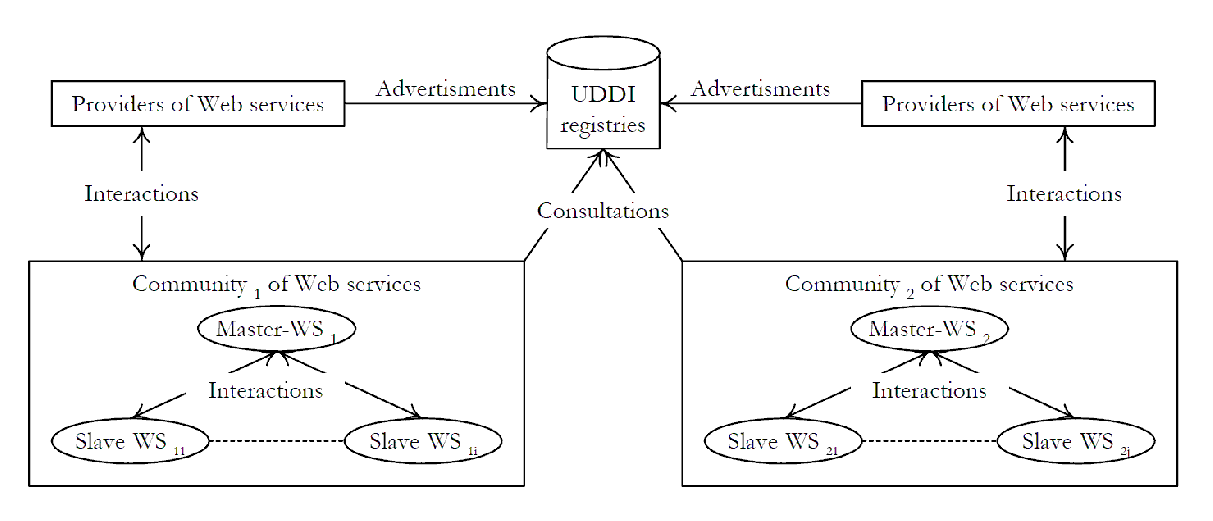
\includegraphics[width=16cm]{Figures/wsarch.eps}\label{wsarch}
            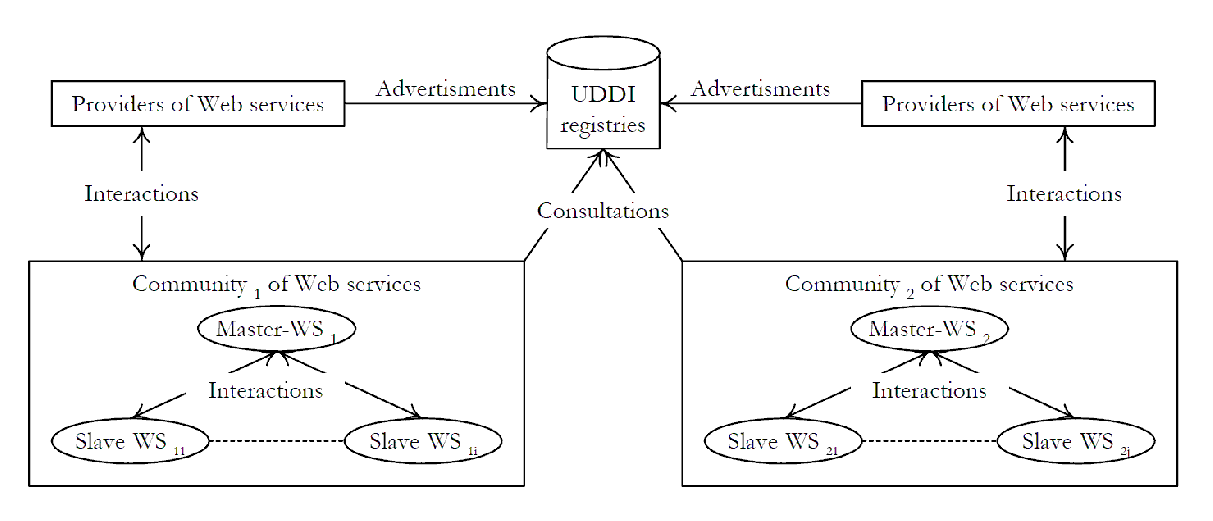
\includegraphics[width=16cm]{Figures/wsarch.eps}\label{wsarch}
            \caption{Communities of Web Services Architecture as Proposed in \cite{DBLP:journals/ijebr/MaamarSTBB09}}
            \end{center}
        \end{figure}

Figure 1 %\ref{wsarch}
depicts the basic architecture of
communities of web services. The main components of the
architecture are: 1) the providers of web services; 2) UDDI
registries; and 3) communities platform. Communities abstract the
same model of defining, announcing and invoking web services. They
also adopt the same protocols that standard web services use with
UDDI registries. UDDI is a platform-independent XML based registry
list which facilitates worldwide web service discovery.

%The master web service is responsible with communication with web
%service providers and discovery registries. It it responsible for
%task distribution, web service selection, community management,
%maintaining a healthy set of web services satisfying end users
%requests with high QoS. In communities, the masters web services
%can be dedicated web services playing the master role during the
%entire time of being in the community. This master web service is
%independently developed and never participates in any
%composition. The master web services can also be chosen out of
%normal web services already inside the community
%\cite{DBLP:journals/ijebr/MaamarSTBB09}.


\section{Cooperative Game Theory and Multi-Agent Systems}\label{sec:CGTMS}

%        Cooperative game theory provides a set of mathematical and optimization tools for multi-agent environments. These tools have been utilized in communication networks and service oriented computing literature, where nodes as rational agents try to reason strategically and maximise their benefit.

Cooperative game is a branch of game theory that studies
strategies of self-interested entities or agents in a setting
where those agents can increase their payoff by binding agreements
and cooperating in groups. We let $N$ be a set of players which
can form a group called a $coalition$. A \emph{coalitional game}
is a pair $G = (N, v)$, where $v$ is called a \emph{characteristic
function} $v: 2^N \to \mathbb{R}$, mapping the set of players of
the coalition to a real number $v(N)$, the worth of $N$. This
number usually represents the output or payoff or again the
performance of these players working together as coalition. If a
coalition $S$ is formed, then it can divide its worth, $v(N)$ in
any possible way among its members. The payoff vector $x \in
\mathbb{R}^N$ is the amount of payoff being distributed among the
members of the coalition $N$. The payoff vector satisfies two
conditions:

        \begin{itemize}
            \item $x_i \geq 0$ for all $i \in N$, and
            \item $\sum_{i \in N} x_i \leq v(N)$
        \end{itemize}

        The second criteria is called the \emph{feasibility} condition,
        according to which, the payoff for each agent cannot be more than
        the coalition total gain. A payoff vector is also \emph{efficient}
        if the payoff obtained by a coalition is distributed amongst the
        coalition members: $\sum_{i \in N} x_i = v(N)$. This definition of
        the characteristic function works in \emph{transferable utility}
        (TU) settings, where utility (i.e., payoff) is transferable from
        one player to another, or in other words, players have common
        currency and a unit of income that is worth the same for all players
        \cite{myerson1991game}.


        \subsection{Cooperative Game Concepts}


            {\bf Definition 1 (Shapley value)} Given a cooperative game $(N,
            v)$, the \emph{Shapley value} of player $i$ is given by \cite{shapley_value}:
            \begin{equation}\label{eq:shapley}
            \phi_i(N,v) = \sum_{S \subseteq N \backslash \left\{i\right\} }
            \frac{|S|! (|N|-|S|-1)!}{|N|!} (v(S \cup \left\{i\right\}) - v(S))
            \end{equation}

            \emph{Shapley value} is a unique and fair solution concept for
            payoff distribution among the members of the coalition. It
            basically rewards members with the amount of marginal contribution
            they have to the coalition.  It checks the contribution of member $i$ by adding the agent, to all possible subsets
            of coalitions $S$, where $S \subseteq N\backslash\left\{i\right\}$. If he is added to the set $S$, his
            contribution to the coalition is $v(S \cup \left\{i\right\}) - v(S)$. Average marginal contribution of agent $i$'s
            is calculated by averaging this value over all possible subsets of $N$, in $Shapley value$ equation (\ref{eq:shapley}).

            %\subsubsection{Core}

            {\bf Definition 2 (Core)} A payoff vector $x$ is in the $core$ of
            a coalitional game $(N, v)$ if and only if:
            \begin{equation}\label{eq:core}
            \forall S \subseteq N, \sum_{x_i \in S} x_i \geq v(S)
            \end{equation}

            The core is basically a set of payoff vectors where no subset of
            players $S^\prime$ could gain more than their current payoff by
            deviating and making their own coalition $\sum_{i \in S^\prime}
            x_i \geq v(S^\prime)$. The sum of payoffs of the players in any
            sub-coalition $S$ is at least as large as the amount that these
            players could earn by forming a coalition by their own. In a
            sense, it is analogue to Nash equilibrium, except that core is
            about deviations from groups of entities. The core is the
            strongest and most popular solution concept in cooperative game
            theory. However, its computation is a combinatorial problem and
            becomes intractable as the number of players increases. The core
            of some real-world problem games may be empty, which means having
            the characteristic function of the game $(N,v)$, there might be no
            possible distribution of payoff assuring stability of subgroups.

            {\bf Definition 3 (Convex cooperative games)} A game $(N,v)$ with
            characteristic function $v(S)$ is convex if:
            \begin{equation}\label{eq:convex}
            v(S) + v(T) \leq v(S \cup T) + v (S \cap T), \forall S,T \subseteq
            N.
            \end{equation}

            According to a classic result by Shapley \cite{S1971cores}, convex
            games always have a non-empty core. We will use a variation of
            convexity condition in our algorithm to check whether our
            coalitions are stable.

            %\subsubsection*{$\epsilon$-core}\label{s:epsilon}
%            %\emph{$\epsilon$-Core:}
%            %\\
%            When the \emph{core} set of a game is empty, it means no coalition
%            of players can gain anything by deviating. An outcome would be
%            unstable if a coalition can benefit even by a small amount from
%            deviating, which is a strong requirement. In fact, in some
%            situations, deviations can be costly, or players may have loyalty
%            to their coalitions, or even it can be computationally intractable
%            to find those small benefits. It would only make sense for a
%            coalition to deviate if the gain from a deviation exceeds the cost
%            of performing the deviation. \emph{$\epsilon$-core} relaxes the
%            notion of the core, and only requires that no coalition would
%            benefit significantly, or within a constant amount($\epsilon$) by
%            deviating (see Equation \ref{eq:core}).
%
%            \begin{equation}\label{eq:core2}
%            \forall S \subseteq N, \sum_{x_i \in S} x_i \geq v(S) - \epsilon
%            \end{equation}

            \subsubsection*{Coalition Structure Formation}\label{sec:coalition}

            Coalition structure formation is the problem of finding the best
            partition of web services into teams. In these settings, the
            performance of an individual service is less important than the
            \emph{social welfare} of the whole system, which is the sum of the
            values of all teams. Having the game $(N,v)$, a coalition
            structure $(CS)$ is \emph{socially optimal} if $CS$ belongs to set
            $\operatorname*{arg\,max}_{CS} v(CS)$ where $v(CS)$ is the sum of
            the values of all coalitions inside $CS$. $v(CS) = \sum_{C \in
            CS}v(C)$.
            %The outcome of a characteristic function game in coalition structure settings, consists of two parts; first a disjoint partition of players (agents) into coalitions, called a \emph{coalition structure} (CS) and second a \emph{payoff vector} as mentioned in cooperative game solution concepts, which distributes the value of each coalition among its members.


        \subsection{Representation and Complexity Issues}\label{sec:CWSArchitecture}

        Shapely value is the unique ``fair'' way to distribute the total surplus generated by the coalition, among all the players.
        The nature of the Shapley value is combinatorial, as all possible orderings to form a
        coalition needs to be considered. This computational complexity can sometimes be
        an advantage as agents cannot benefit from manipulation. For example, it is NP-complete
        to determine whether for a bunch of agents to collude and make their own coalition and guarantee
        an increase in payoff of all participants \cite{conf/aaai/YokooCSOI05}.
        There are some representations that allow us to compute the Shapley value efficiently by reducing the input size of the problem.
        One example is \emph{Induced subgraph games}
        which was introduced by Deng and Papadimitriou \cite{Deng94}. In this representation, players are represented by graph nodes, and
        their valuation function should be the sum of weights of all edges between the node and all its neighbors. It is a succinct representation, using
        an adjacency matrix, which needs only $O(n^2)$ space to store all the input, which is a major improvement from $O(2^n)$ because
        if weights of all the edges in graph are all positive, the Shapley value can be computed in time $O(n^2)$.
        However, this representation is not complete, some games cannot be represented by a induced subgraph game \cite{conf/aaai/YokooCSOI05}.

        Ketchpel introduces the Bilateral Shapley Value (BSV) \cite{conf/aaai/Ketchpel94a} for coalition games with general valaution functions.
        It reduces the combinatorial complexity of the computation of the Shapley value, breaking the community to multiple disjoint set.
        With backtracking and dynamic programming like methods, they merge and store the marginal contribution of disjoint coalitions,
        reducing the overall complexity of the algorithm. However, the solution is still NP-Complete and BSV time and space complexity grows exponentially.

        In order to make cooperative game concepts practical in real world application, we have proposed an approximation multi-layer
        algorithm useful for service oriented computing settings. Our excrements illustrate, these algorithms can provide
        applicable and near optimal solutions for real world applications.

\subsection{Stability of Coalitions}

Core stability is a highly desirable property however in many problems it is not achievable. It would be more ideal to maintain a set of somewhat stable payoffs when the core is empty. There are several approaches to achieve this goal. One may drop the stability requirement and focus on other types of solutions for which a payoff division is guaranteed to exist. Two well known solution concepts in this category are \emph{nucleolus}\cite{schmeidler_nucleolus_1969} and the \emph{bargaining set}\cite{Davis67existenceof}. They try to minimize some measure of unhappiness in the game for the agents.

Another approach to stabilize the game can be achieved via external subsides. When \emph{Core} is empty it means the game is not stable since the coalition is unable to generate enough revenue to satisfy the demands of each subset of agents. An external party that is interested in stabilizing the game provides a subsidy to the agents if they form the grand coalition, and thus a value of $\lambda v(C)$ is divided among them, where $\lambda \geq 1$. Clearly any game can be stabilized using a large enough $\lambda$, however the external party would be interested in the minimal subsidy required in order to stabilize the game.

A community can also be stabilized by relaxing the core constraints. According to \emph{Core}, an outcome is unstable if a coalition can benefit even by a small amount from deviating, which is a strong requirement. In fact, in some situations, deviations can be costly, or players may have loyalty to their coalitions, or even it can be computationally intractable to find those small benefits. It would only make sense for a coalition to deviate if the gain from a deviation exceeds the cost of performing the deviation. \emph{$\epsilon$-core} relaxes the notion of the core, and only requires that no coalition would benefit significantly, or within a constant amount($\epsilon$) by deviating (see Equation \ref{eq:core}). 

   \begin{equation}\label{eq:core2}
       \forall S \subseteq N, \sum_{x_i \in S} x_i \geq v(S) - \epsilon
   \end{equation}
   
Alternatively, the $\epsilon$ can be thought of as a \emph{tax} imposed on a coalition should it choose to deviate. This can again be seen as an external party, trying to stabilize the coalition by imposing some \emph{tax} on deviation. Taxation and subsiding as methods of stabilizing cooperative games have been studied in \cite{RePEc:spr:jogath:v:38:y:2009:i:1:p:3-16, RePEc:mse:cesdoc:12022r, Bachrach:2009:CSC:1692490.1692502, conf/ijcai/MeirRM11}.



\section{Related Work}\label{sec:BRRelatedWork}

The idea of grouping web services within virtual structures was
fist proposed by Zeng et al. \cite{Zeng:2003:QDW:775152.775211}.
The authors defined web service community as collection of web
services providing the same functionality, but with different
quality metrics. Medjahed and Boubuettaya
\cite{journals/dpd/MedjahedB05} have proposed a framework and a
community builder mechanism which uses semantic analysis,
providing an ontological organization of web services having the
same domain of interest. The community builder would suggest web
services having similar operations to join the same community, or
form their own community in case the semantic analysis cannot find
any community that matches the service types.

        Most of the recent work on communities of services are either
        user-centric and focus on user satisfaction
        \cite{Chun02user-centricperformance} or system-centric and focus
        on the whole system throughput, performance and utilization. There
        are many contributions in distributed, grid, cluster and cloud
        services which are system-centric. However, in real world
        environments and applications, both users and service providers
        are self-interested agents, aiming to maximize their own profit.
        In those environments, both parties (users and services) will
        collaborate as long as they are getting more benefits and payoff.

        In this direction, recently \cite{DBLP:conf/IEEEscc/LimTMB12,
        DBLP:conf/IEEEscc/KhosravifarABT11, 10.1109/TSC.2012.12} proposed mechanisms to help
        users and services maximize their gain. A two-player
        non-cooperative game between web services and community master was
        introduced in \cite{DBLP:conf/IEEEscc/KhosravifarABT11}. In this
        game-theoretic model, the strategies available to a web service
        when facing a new community are requesting to join the community,
        accepting the master's invitation to join the community, or
        refusing the invitation to join. The set of strategies for
        communities are inviting the web service or refusing the web
        service's join request. Based on their capacity, market share and
        reputation, the two players have different set of utilities over
        the strategy profiles of the game. The main limits of this game
        model are: 1) its consideration of only three quality parameters,
        while the other factors are simply ignored; and 2) the
        non-consideration of the web services already residing within the
        community. The game is only between the community master and the
        new web service, and the inputs from all the other members are
        simply ignored. The consideration of those inputs is a significant
        issue as existing web services can lose utility or payoff because
        of the new member, which can results in an unhealthy and unstable
        group. The problem comes from the fact that the existing members
        should collaborate with the new web services, so probably their
        performance as a group can suffer. Existing members may even
        deviate and try to join other communities if they are unsatisfied.
        Those considerations of forming stable and efficient coalitions
        are the main contributions of this research work.

        In \cite{DBLP:conf/IEEEscc/LimTMB12}, a 3-way satisfaction approach
        for selecting web services has been proposed. In this approach,
        the authors proposed a web service selection process that the
        community masters can use. The approach considers the efficiency
        of all the three involved parties, namely users, web services and
        communities. In this work, it is shown how the gains of these
        parties are coupled together using a linear optimization process.
        However, the optimization problem in this solution tends to
        optimize some parameters considering all web services regardless
        of their efficiency and contribution to the community's welfare.
        Moreover, there are no clear thresholds for accepting or rejecting
        new web services. The solution of the optimization problem could,
        for instance, suggest web services already residing within the
        community to increase or decrease their capacity to cover up the
        weakness of other parties in the system. However, a high
        performing web service could deviate anytime it finds itself
        unsatisfied within the community instead of adjusting its service
        parameters.

        In \cite{10.1109/TSC.2012.12}, a cooperative scheme among autonomous
        web services based on coalitional game theory has been introduced. The authors have proposed an algorithm to
        reach individually stable coalition partition for web services in order to
        maximize their efficiency. The communities choose new web services on the promise
        that it would benefit the community without decreasing any other web service's
        income. In their model, the worth of community is evaluated with high emphasis on
        availability metric and considering price and cost values only. The community structure is based on a coordination chain,
        where a web service is assigned as a \emph{primary} web service and the community task destribution
        method, will initially invoke the primary web service and only if the primary web service is unavailable
        will invoke the next backup web services as they are ordered in the coordination chain. However in cooperative models, it is preferred to
        have a real and active cooperative activity engaging all agents to perform the tasks more efficiently. Especially nowadays
        with recent advancement in cloud and hardware infrastructures availability is becoming less of an issue. So the backup web services
        in their model have a very low chance of getting jobs, especially the ones further in chain, which is huge waste of web services
        capabilities.

\section{Conclusive Remarks}


        In this research work, we will use game theory to
        propose a cooperative game model for the aggregation of web
        services within communities. The solution concepts of our
        cooperative game seeks to find efficient ways of forming
        coalitions (teams) of web services so that they can maximize their
        gain and payoff, and distribute the gain in a fair way among all
        the web services. Achieving Fairness when the gain is distributed
        among the community members is the main factor to keep the
        coalition stable as no web service will expect to gain better by
        deviating from the community. In other words, the coalition is made
        efficient if all the members are satisfied. We first propose a
        representation function for communities of web services based on
        their QoS attributes. By using this function, we can evaluate the
        $worth$ of each community of web services. When facing new
        membership requests, a typical community master checks whether the
        new coalition having the old and new set of web services will keep
        the community stable or not. The community master will reject the
        membership requests if it finds out that the new coalition would
        be unstable, preventing $any$ subset of web services from gaining
        significantly more by deviating from the community and joining
        other communities or forming new ones. The computation of
        solutions for cooperative game theory problems is combinatorial in
        nature and proven to be NP-complete \cite{Algorithmic}, making
        this computation impractical in real world applications. However,
        using the concepts of coalition stability, we propose
        approximation algorithms running in polynomial time providing web
        services and community masters with applicable and near-optimal
        decision making mechanisms.




%*******************************End Background **********************************
